%%%%%%%%%%%%%%%%%%%%%%%%%%%%%%%%%%%%%%%%%
% Focus Beamer Presentation
% LaTeX Template
% Version 1.0 (8/8/18)
%
% This template has been downloaded from:
% http://www.LaTeXTemplates.com
%
% Original author:
% Pasquale Africa (https://github.com/elauksap/focus-beamertheme) with modifications by 
% Vel (vel@LaTeXTemplates.com)
%
% Template license:
% GNU GPL v3.0 License
%
% Important note:
% The bibliography/references need to be compiled with bibtex.
%
%%%%%%%%%%%%%%%%%%%%%%%%%%%%%%%%%%%%%%%%%

%----------------------------------------------------------------------------------------
%	PACKAGES AND OTHER DOCUMENT CONFIGURATIONS
%----------------------------------------------------------------------------------------

\documentclass{beamer}

\usetheme{focus} % Use the Focus theme supplied with the template
% Add option [numbering=none] to disable the footer progress bar
% Add option [numbering=fullbar] to show the footer progress bar as always full with a slide count

% Uncomment to enable the ice-blue theme
\definecolor{main}{RGB}{42,56,144}
\definecolor{background}{RGB}{240, 247, 255}
\definecolor{bluenight}{RGB}{42,56,143}
\definecolor{skyblue}{RGB}{126,233,233}
\usepackage{algorithm2e}
\usepackage{textcomp}

\usepackage[T1]{fontenc}
%------------------------------------------------
\newtheorem{prop}{Lemma}
\usepackage{booktabs} % Required for better table rules
\setbeamerfont{frametitle}{size=\large}
\usepackage{xcolor}
\usetikzlibrary{shadings,shadows,shapes.arrows}
\usepackage{tikz}
\usetikzlibrary{positioning}% To get more advances positioning options
\DeclareMathOperator{\tr}{Tr}
\usepackage{listings}
\usepackage{color}
\definecolor{lightgray}{gray}{0.9}
\makeatletter
\newcommand{\srcsize}{\@setfontsize{\srcsize}{7pt}{7pt}}
\makeatother
\usepackage[skins,listings,breakable]{tcolorbox}
\usepackage{MnSymbol,wasysym}

\lstset{language=R,
	basicstyle={\ttfamily\small},
	otherkeywords={0,1,2,3,4,5,6,7,8,9},
	morekeywords={TRUE,FALSE},
	deletekeywords={data,frame,length,as,character},
	keywordstyle=\color{bluenight},
	upquote = true
}

\newcommand{\inlinecode}[2]{\colorbox{lightgray}{\lstinline[language=#1]$#2$}}
\usetikzlibrary{arrows}
\newcommand*{\tikzarrow}[2]{%
	\tikz[
	baseline=(A.base),             % Set baseline to the baseline of node content
	font=\footnotesize\sffamily    % Set fontsize of the node content
	]
	\node[
	single arrow,                  % Shape of the node
	single arrow head extend=3pt,  % Actual width of arrow head
	draw,                          % Draw the node shape
	inner sep=5pt,                 % Separation between node content and node shape
	top color=bluenight,               % Shading color on top of node
	bottom color=#1,               % Shading color on bottom of node
	] (A) {#2};%
}
\newcommand*{\tikzarrowD}[2]{%
	\tikz[
	baseline=(A.base),             % Set baseline to the baseline of node content
	font=\footnotesize\sffamily    % Set fontsize of the node content
	]
	\node[
	single arrow,     
	single arrow tip angle=150,    % Adjust arrow tip angle
	shape border rotate=270,       % Rotate the arrow shape to point down             % Shape of the node
	single arrow head extend=6pt,  % Actual width of arrow head
	draw,                          % Draw the node shape
	inner sep=6pt,                 % Separation between node content and node shape
	top color=bluenight,               % Shading color on top of node
	bottom color=#1,               % Shading color on bottom of node
	] (A) {#2};%
}

%----------------------------------------------------------------------------------------
%	 TITLE SLIDE
%----------------------------------------------------------------------------------------
\setbeamerfont{institute}{size=\fontsize{7.5pt}{8.5pt}}
\setbeamerfont{author}{size=\fontsize{12pt}{13pt}}

\title[scale=.1]{pARI package: valid double-dipping via permutation-based All Resolutions Inference}

\author[Angela Andreella]{Angela Andreella\inst{1} \hspace{1cm} Livio Finos\inst{2}  \hspace{1cm}  Jelle Goeman\inst{3}}

\institute[] % (optional, but mostly needed)
{
	\inst{1}%
	Department of Statistical Sciences, University of Padua
	\vspace{1mm}	\\
	\inst{2}%
	Department of Developmental Psychology and Socialisation, University of Padua  \\
	\inst{3}%
	Biomedical Data Sciences, Leiden University Medical Center  \\
	
}
\date{useR! - 6 July 2021 }
\titlegraphic{\vspace{2.3cm} 
\includegraphics[scale=.12]{Images/s4.png}}

%------------------------------------------------

\begin{document}

%------------------------------------------------

\begin{frame}
	\maketitle % Automatically created using the information in the commands above
\end{frame}

%------------------------------------------------

\begin{frame}{Motivation - fMRI data}

fMRI measures brain activation as changes in blood flow (BOLD) under a sequence of stimuli. 
\vspace{.4cm} 

\textcolor{bluenight}{\textbf{Cluster-wise method}}:

\begin{itemize}
	
	\item Analyze set of contiguous voxels (S);
	\vspace{.4cm} 
	\item  $H_S$ rejected means that $S$ contains at least one active voxel $\rightarrow$ We don't know which ones and how many!!
	\vspace{.4cm}  
	\item \textcolor{black}{\textbf{Spatial specificity paradox}};
	\vspace{.4cm} 
	\item \textcolor{black}{\textbf{Double-dipping}}.
\end{itemize}

\end{frame}

\begin{frame}{ARI and pARI}

\textcolor{bluenight}{\textbf{Solution}}: All-resolutions inference (ARI) \footnotemark \footnotetext[1]{Resenblatt, J. et al. (2018).} $\rightarrow$ Inference on the number of truly active voxels.

\vspace{.4cm}

\begin{itemize}
	\item \textcolor{bluenight}{\textbf{pARI}} is the Permutation-based version of \textcolor{bluenight}{\textbf{ARI}}. The permutation structure permits to account for the correlation structure between tests unlike \textcolor{bluenight}{\textbf{ARI}};
	\vspace{.4cm}
	\item Both methods are based on the \textcolor{bluenight}{\textbf{closed testing procedure}} for controlling the familywise error rate.
\end{itemize}



\end{frame}

\begin{frame}{Not only fMRI data!}

Every time that we want to infer inside a \textcolor{bluenight}{\textbf{data-driven (and not) cluster}} (features set), we can use \textcolor{bluenight}{\textbf{ARI/pARI}}:
\vspace{.5cm}
\begin{itemize}
	\item \textcolor{bluenight}{\textbf{Cluster fMRI data analysis}} \footnotemark \footnotetext[2]{Woo, C. et al. (2014).};
	\vspace{.5cm}
	\item \textcolor{bluenight}{\textbf{Gene expression cluster analysis}} \footnotemark \footnotetext[3]{Berge, K. et al. (2017).};
	\vspace{.5cm}
	\item \textcolor{bluenight}{\textbf{Cluster EEG data analysis}} \footnotemark \footnotetext[4]{Maris, E. et al. (2007).}.
\end{itemize}

\end{frame}



\begin{frame}[fragile]{Main functions of pARI}

\begin{tcblisting}{breakable,listing only,
		listing options={language=c,aboveskip=0pt,belowskip=0pt},
		size=fbox,boxrule=0pt,frame hidden,arc=0pt,colback=lightgray}
devtools::install_github(angeella/pARI)
library(pARI)
\end{tcblisting}

\begin{itemize}
	\item fMRI framework: \begin{tcblisting}{breakable,listing only,
			listing options={language=c,aboveskip=0pt,belowskip=0pt},
			size=fbox,boxrule=0pt,frame hidden,arc=0pt,colback=lightgray}
	pARIbrain(copes, thr, mask, alpha, ...)
	\end{tcblisting}
where \colorbox{skyblue}{\texttt{copes}} is a list of \textcolor{bluenight}{\textbf{contrast}} parameter estimates involving brain activation differences for each subject in NIfTI format.
	\item General framework: \begin{tcblisting}{breakable,listing only,
			listing options={language=c,aboveskip=0pt,belowskip=0pt},
			size=fbox,boxrule=0pt,frame hidden,arc=0pt,colback=lightgray}
	pARI(data, ix, alpha, test.type, ...)
	\end{tcblisting}
where \colorbox{skyblue}{\texttt{ix}} is the \textcolor{bluenight}{\textbf{features set}} of interest. It can be a vector of indices or a vector with length equals the number of features where different values indicate the different sets.
\end{itemize}



\end{frame}

%\begin{frame}[fragile]{Toy example}
%Let simulate some simple data as
%\begin{align*}
%\mathbf{Y}_i = \boldsymbol{\mu} + \boldsymbol{\epsilon}_i \quad\quad \text{where} \quad \boldsymbol{\epsilon}_i \sim \mathcal{N}(0,\Sigma_{\rho^2}).
%\end{align*}
%
%
%\begin{tcblisting}{breakable,listing only,
%		listing options={language=c,aboveskip=0pt,belowskip=0pt},
%		size=fbox,boxrule=0pt,frame hidden,arc=0pt,colback=lightgray}
%DB <- simulateData(m = 2000, n = 10, rho = 0, 
%                   pi0 = 0.8, power = 0.8)
%pARI(data = DB, ix = c(1:100), alpha = 0.05, 
%type.test = "one_sample")
%81
%\end{tcblisting}
%We can say that \textcolor{bluenight}{\textbf{at least}} $81$ features in the set \texttt{ix}, i.e., the first $100$ features, are true discoveries.
%\end{frame}

\begin{frame}[fragile]{fMRI data Application - Code}
We analyzed the \textcolor{bluenight}{\textbf{Auditory data}} collected by Pernet et al. (2015), i.e, people listening vocal and non-vocal sounds. 
\vspace{.2cm}

Group analysis on $140$ subjects of the Vocal $>$ Non-vocal \textcolor{bluenight}{\textbf{contrast}} by the one sample t-test flipping the sign of $140$ voxel-wise contrasts maps. 
\vspace{.5cm}

First, let download the data from the \texttt{fMRIdata} package:

\vspace{.5cm}
\begin{tcblisting}{breakable,listing only,
		listing options={language=r,aboveskip=0pt,belowskip=0pt},
		size=fbox,boxrule=0pt,frame hidden,arc=0pt,colback=lightgray}
devtools::install_github(angeella/fMRIdata)
library(fMRIdata)
data(Auditory_clusterTH3_2)
data(Auditory_copes)
data(Auditory_mask)
\end{tcblisting}

\end{frame}

\begin{frame}[fragile]{fMRI data Application - Code}

\begin{tcblisting}{breakable,listing only,
		listing options={language=c,aboveskip=0pt,belowskip=0pt},
		size=fbox,boxrule=0pt,frame hidden,arc=0pt,colback=lightgray}
pARIbrain(copes = Auditory_copes, 
          cluster = Auditory_clusterTH3_2,
          mask = Auditory_mask, 
          alpha = 0.05)
\end{tcblisting}


\end{frame}


\begin{frame}{fMRI data Application - Results}
\begin{table}
	\begin{tabular}{@{}rlrrrc@{}}
		\hline
		\multicolumn{1}{c}{\textcolor{bluenight}{\textbf{Cluster}}} &\multicolumn{1}{c}{\textcolor{bluenight}{\textbf{Threshold}}} & \multicolumn{1}{c}{\textcolor{bluenight}{\textbf{Size}}} &\multicolumn{2}{c}{\textcolor{bluenight}{\textbf{$\%$ active}}}& \multicolumn{1}{c}{\textcolor{bluenight}{\textbf{P-Values}}}  \\
		\multicolumn{1}{c}{$S$}&\multicolumn{1}{c}{$t$}  &\multicolumn{1}{c}{$|S|$} & \multicolumn{2}{c}{$\bar{\pi}(S)$}&\multicolumn{1}{c}{$p_{FWER}$}  \\ 
		&  &&pARI  & ARI &   \\ 
		\hline
		Right STG/PT &$3.2$ &$11683$  &   \colorbox{pink}{$92.36\%$} &   $84.98\%$ &$<0.0001$\\
		HG/IFG/T & &      &   &  &\\
		Right STG/PT &$4$ &$8875$  &   $99.54\%$ &   $98.5\%$ &$-$\\
		HG/IFG/T & &  &      &  &\\
		Right IFG &$4$ &$422$  &   $91.47\%$ &   $83.18\%$ &$-$ \\
		Right T & $4$ &  $292$  & $85.96\%$&  $64.04\%$ & $-$\\
		Right T & $4$ &  $15$  & $13.33\%$&  $0\%$ & $-$\\
	\end{tabular}
\end{table}
\end{frame}

\begin{frame}{fMRI data Application - Results}
\texttt{map\_TDP}: Create \textcolor{bluenight}{\textbf{true discovery proportion map}} in nifti format.
\vspace{1cm}
\begin{figure}
	\centering
	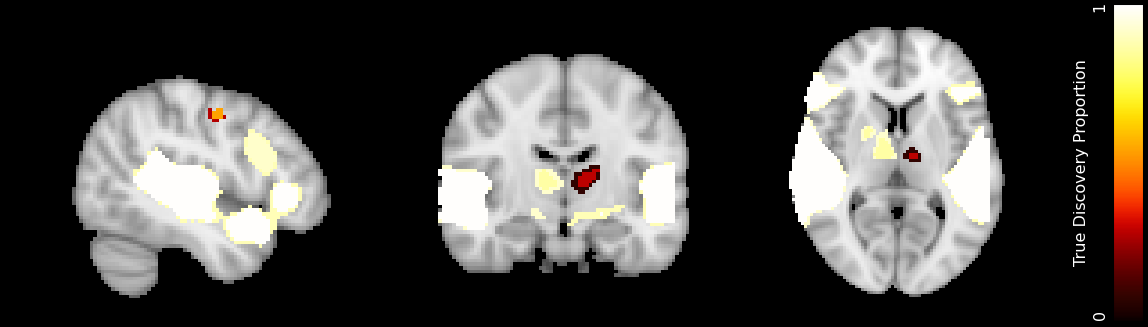
\includegraphics[width=\textwidth]{Images/Auditory_tdp.png}
\end{figure}
\end{frame}

\begin{frame}
Thanks to the amazing group that worked on the paper \emph{Permutation-based true discovery proportions for fMRI cluster analysis}! (in arXiv)

\begin{itemize}
	\item Livio Finos \hspace{.2cm} University of Padua;
	\item Jelle Goeman \hspace{.2cm} Leiden University Medical Centre;
	\item Jesse Hemerik \hspace{.2cm} Wageningen University;
	\item Wouter Weeda \hspace{.2cm} Leiden University;
\end{itemize}

\begin{center}
	and thanks for your attention!
\end{center}


\includegraphics[width=.048\textwidth]{Images/Githu.png} angeella 

\vspace{.4cm}


\includegraphics[width=.04\textwidth]{Images/twitter.png} @aangeella

\vspace{.4cm}


\includegraphics[width=.04\textwidth]{Images/email.png} angela.andreella@stat.unipd.it


\end{frame}


\end{document}
